\section{Appendix}

\subsection{Word Count}
\detailtexcount{main}\~13000

\subsection{Dissertation Structure}
\begin{figure}[H]
	\centering
	\usetikzlibrary{shapes.geometric, positioning}
	\tikzstyle{bk} = [rectangle, draw, text centered, rounded corners, font=\scriptsize]
	\tikzstyle{bk2} = [rectangle, draw, text centered, rounded corners]
	\tikzstyle{tz} = [trapezium, draw, rounded corners, text centered, fill=blue!20, trapezium stretches=true]
	\tikzstyle{tz2} = [trapezium, draw, rounded corners, text centered, font=\scriptsize,trapezium angle = -45, trapezium stretches=true]
	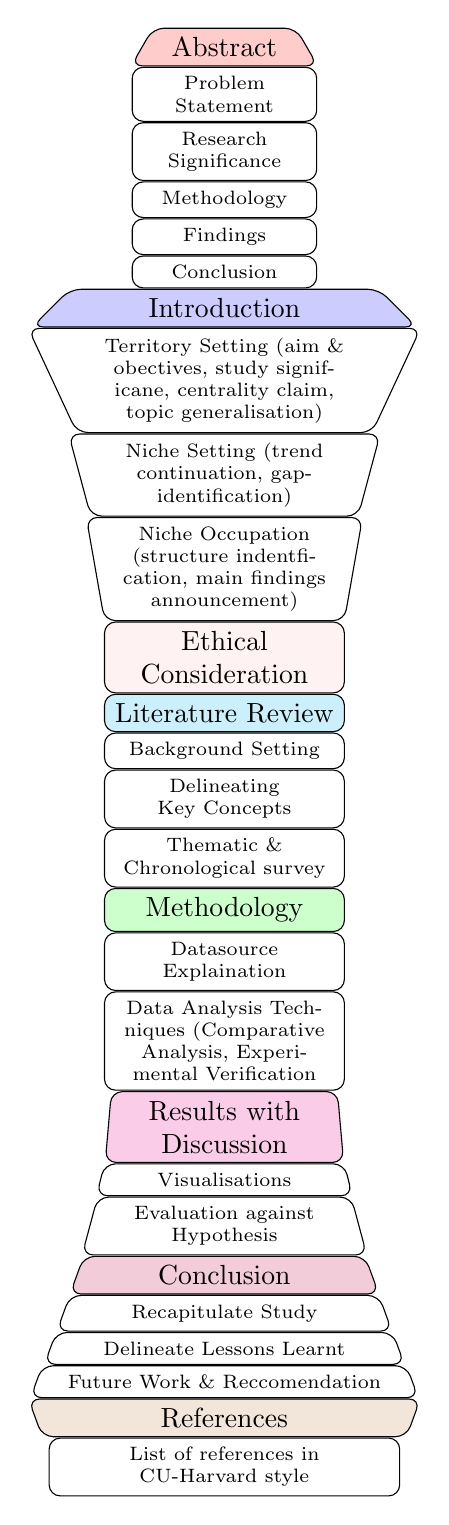
\begin{tikzpicture}[node distance=0.1pt]
	\node [tz, text width=4.5em, fill=red!20] (a) {Abstract};
	\node [bk, below = of a, text width=6em] (p) {Problem Statement};
	\node [bk, below = of p, text width=6em] (r) {Research\\ Significance};
	\node [bk, below = of r, text width=6em] (m) {Methodology};
	\node [bk, below = of m, text width=6em] (f) {Findings};
	\node [bk, below = of f, text width=6em] (c) {Conclusion};
	\node [tz, below = of c, trapezium angle = 45, text width=10.5em] (i) {Introduction};
	\node [tz2, below = of i, text width=10em, trapezium angle = -65] (t) {Territory Setting (aim \& obectives, study significane, centrality claim, topic generalisation)};
	\node [tz2, below = of t, text width=9em, trapezium angle = -75](n) {Niche Setting (trend continuation, gap-identification)};
	\node [tz2, below = of n, text width=8em, trapezium angle= -80] (no) {Niche Occupation (structure indentfication, main findings announcement)};
	\node [bk2, below = of no, text width=8em, trapezium angle= 90, fill=pink!20] (ep) {Ethical\\ Consideration};
	\node [bk2, below = of ep, text width=8em, trapezium angle= 90, fill=cyan!20] (l) {Literature Review};
	\node [bk, below = of l, text width=8em, trapezium angle= 90] (bs) {Background Setting};
	\node [bk, below = of bs, text width=8em, trapezium angle= 90] (dk) {Delineating Key Concepts};
	\node [bk, below = of dk, text width=8em, trapezium angle= 90] (ta) {Thematic \&\\ Chronological survey};
	\node [bk2, below = of ta, text width=8em, trapezium angle= 90, fill=green!20] (me) {Methodology};
	\node [bk, below = of me, text width=8em, trapezium angle= 90] (de) {Datasource Explaination};
	\node [bk, below = of de, text width=8em, trapezium angle= 90] (te) {Data Analysis Techniques (Comparative Analysis, Experimental Verification};
	\node [tz, below = of te, text width=7.5em, trapezium angle= 85, fill=magenta!20] (rd) {Results with Discussion};
	\node [tz2, below = of rd, text width=8em, trapezium angle= 76] (vi) {Visualisations};
	\node [tz2, below = of vi, text width=8.5em, trapezium angle= 75] (eh) {Evaluation against Hypothesis};
	\node [tz, below = of eh, text width=9.5em, trapezium angle= 70, fill=purple!20] (co) {Conclusion};
	\node [tz2, below = of co, text width=10.5em, trapezium angle= 70] (rt) {Recapitulate Study};
	\node [tz2, below = of rt, text width=11.5em, trapezium angle= 70] (ll) {Delineate Lessons Learnt};
	\node [tz2, below = of ll, text width=12.5em, trapezium angle= 70] (fr) {Future Work \& Reccomendation};
	\node [tz, below = of fr, text width=12.5em, trapezium angle=-70, fill=brown!20] (re) {References};
	\node [tz2, below = of re, text width=12em, trapezium angle= 90] (rd) {List of references in CU-Harvard style};
	\end{tikzpicture} 
	\caption{Custom-designed ordered Structure for my Dissertation}
\end{figure}

\subsection{Visual Classification Scheme}
\begin{figure}[H]
	\centering
	\includegraphics[width=\linewidth, height=\textheight, keepaspectratio]{images/tree.jpg}
	\caption{Galaxy Zoo Decision Tree for Visual Classification}
\end{figure}
\newpage
\subsection{Code Snippets}
\subsection{GUI Prototype}
The system developed does not have a graphical user interface. It uses command-line user interface. I have however developed a prototype for the GUI using the Django web-framework. The file structure is shown in figure \ref{fig:dvs} The CLI routines are integrated into the view controllers in Django as shown in figure \ref{fig:dvc_1} and \ref{fig:dvc_2}. The corresponding source code of the rendered page is shown in figure \ref{fig:dvt1} and \ref{fig:dvt2}. The rendered page itself is shown in figure \ref{fig:dvg}

\begin{figure}[H]
	\centering
	\includegraphics[width=.3\linewidth, height=\textheight, keepaspectratio]{images/code/dvs.png}
	\caption{File structure for the GUI prototype developed in Django.}
	\label{fig:dvs}
\end{figure}

\begin{figure}[H]
	\centering
	\frame{\includegraphics[width=\linewidth, keepaspectratio]{images/code/dvt_1.png}}
	\caption{An example of front-end design with HTML and Django Template (Part 1 of 2).}
	\label{fig:dvt1}
\end{figure}
\begin{figure}[H]
	\centering
	\frame{\includegraphics[width=\linewidth, keepaspectratio]{images/code/dvt_2.png}}
	\caption{An example of front-end design with HTML and Django Template (Part 2 of 2).}
	\label{fig:dvt2}
\end{figure}
\begin{figure}[H]
	\centering
	\frame{\includegraphics[width=\linewidth, keepaspectratio]{images/code/dvc_1.png}}
	\caption{An example of view controller with routines integrated in Django (Part 1 of 2).}
	\label{fig:dvc_1}
\end{figure}
\begin{figure}[H]
	\centering
	\frame{\includegraphics[width=\linewidth, keepaspectratio]{images/code/dvc_2.png}}
	\caption{An example of view controller with routines integrated in Django. (Part 2 of 2)}
	\label{fig:dvc_2}
\end{figure}
\begin{figure}[H]
	\centering
	\frame{\includegraphics[width=\linewidth, keepaspectratio]{images/gui.png}}
	\caption{Sample page loaded with Django controllers as part of GUI prototype.}
	\label{fig:dvg}
\end{figure}

\subsection{Redshift Regression}
\begin{figure}[H]
	\centering
	\frame{\includegraphics[width=.4\linewidth, height=\textheight, keepaspectratio]{images/code/dvs_2.png}}
	\caption{File structure of classification and regression on SDSS dataset.}
	\label{fig:dvs_2}
\end{figure}
\begin{figure}[H]
	\centering
	\frame{\includegraphics[width=.7\linewidth, height=\textheight, keepaspectratio]{images/code/r1.png}}
	\caption{Features (u,g,r,i,z flux magnitudes) Extraction from SDSS dataset.}
	\label{fig:r1}
\end{figure}
\begin{figure}[H]
	\centering
	\frame{\includegraphics[width=.7\linewidth, height=\textheight, keepaspectratio]{images/code/r2.png}}
	\caption{Training the decision tree regressor.}
	\label{fig:r2}
\end{figure}
\begin{figure}[H]
	\centering
	\frame{\includegraphics[width=.7\linewidth, height=\textheight, keepaspectratio]{images/code/r3.png}}
	\caption{Calculating median residuals.}
	\label{fig:r3}
\end{figure}
\begin{figure}[H]
	\centering
	\frame{\includegraphics[width=\linewidth, height=\textheight, keepaspectratio]{images/code/r4_1.png}}
	\caption{Regression with hold-out validation (Part 1 of 2).}
	\label{fig:r4_1}
\end{figure}
\begin{figure}[H]
	\centering
	\frame{\includegraphics[width=\linewidth, height=\textheight, keepaspectratio]{images/code/r4_2.png}}
	\caption{Regression with hold-out validation (Part 2 of 2).}
	\label{fig:r4_2}
\end{figure}
\begin{figure}[H]
	\centering
	\frame{\includegraphics[width=\linewidth, height=\textheight, keepaspectratio]{images/code/r5.png}}
	\caption{Colour vs Colour Redshift Plot.}
	\label{fig:r5}
\end{figure}
\begin{figure}[H]
	\centering
	\frame{\includegraphics[width=\linewidth, height=\textheight, keepaspectratio]{images/code/o1_1.png}}
	\caption{K-Fold Cross-Validated Predictions (Part 1 of 2).}
	\label{fig:o1_1}
\end{figure}
\begin{figure}[H]
	\centering
	\frame{\includegraphics[width=\linewidth, height=\textheight, keepaspectratio]{images/code/o1_2.png}}
	\caption{K-Fold Cross-Validated Predictions (Part 2 of 2).}
	\label{fig:o1_2}
\end{figure}
\begin{figure}[H]
	\centering
	\frame{\includegraphics[width=\linewidth, height=\textheight, keepaspectratio]{images/code/o2_1.png}}
	\caption{K-Fold Cross-Validation (Part 1 of 2).}
	\label{fig:o2_1}
\end{figure}
\begin{figure}[H]
	\centering
	\frame{\includegraphics[width=\linewidth, height=\textheight, keepaspectratio]{images/code/o2_2.png}}
	\caption{K-Fold Cross-Validation(Part 2 of 2).}
	\label{fig:o2_2}
\end{figure}
\begin{figure}[H]
	\centering
	\frame{\includegraphics[width=\linewidth, height=\textheight, keepaspectratio]{images/code/o3_1.png}}
	\caption{Overfitting Trees with varying tree depth (Part 1 of 2).}
	\label{fig:o3_1}
\end{figure}
\begin{figure}[H]
	\centering
	\frame{\includegraphics[width=\linewidth, height=\textheight, keepaspectratio]{images/code/o3_2.png}}
	\caption{Overfitting Trees with varying tree depth (Part 2 of 2).}
	\label{fig:o3_2}
\end{figure}
\begin{figure}[H]
	\centering
	\frame{\includegraphics[width=\linewidth, height=\textheight, keepaspectratio]{images/code/o4.png}}
	\caption{Visualising decision tree regressor trained model with mean squared errors.}
	\label{fig:o4}
\end{figure}
\begin{figure}[H]
	\centering
	\frame{\includegraphics[width=\linewidth, height=\textheight, keepaspectratio]{images/code/o5_1.png}}
	\caption{Quasars vs Galaxy redshift predictions (Part 1 of 2).}
	\label{fig:o5_1}
\end{figure}
\begin{figure}[H]
	\centering
	\frame{\includegraphics[width=\linewidth, height=\textheight, keepaspectratio]{images/code/o5_2.png}}
	\caption{Quasars vs Galaxy redshift predictions (Part 2 of 2).}
	\label{fig:o5_2}
\end{figure}

\subsection{Morphology Classification}
\begin{figure}[H]
	\centering
	\frame{\includegraphics[width=\linewidth, height=\textheight, keepaspectratio]{images/code/c1.png}}
	\caption{Splitting the galaxy catalogue.}
	\label{fig:c1}
\end{figure}
\begin{figure}[H]
	\centering
	\frame{\includegraphics[width=\linewidth, height=\textheight, keepaspectratio]{images/code/c2.png}}
	\caption{Generating features and targets.}
	\label{fig:c2}
\end{figure}
\begin{figure}[H]
	\centering
	\frame{\includegraphics[width=\linewidth, height=\textheight, keepaspectratio]{images/code/c3_1.png}}
	\caption{Training the decision tree classifier (Part 1 of 2).}
	\label{fig:c3_1}
\end{figure}
\begin{figure}[H]
	\centering
	\frame{\includegraphics[width=\linewidth, height=\textheight, keepaspectratio]{images/code/o5_2.png}}
	\caption{Training the decision tree classifier (Part 2 of 2).}
	\label{fig:c3_2}
\end{figure}
\begin{figure}[H]
	\centering
	\frame{\includegraphics[width=\linewidth, height=\textheight, keepaspectratio]{images/code/c4_1.png}}
	\caption{Accuracy and model's score with confusion matrix.}
	\label{fig:c4_1}
\end{figure}
\begin{figure}[H]
	\centering
	\frame{\includegraphics[width=.7\linewidth, height=\textheight, keepaspectratio]{images/code/c4_2.png}}
	\caption{Accuracy and model's score with confusion matrix.}
	\label{fig:c4_2}
\end{figure}
\begin{figure}[H]
	\centering
	\frame{\includegraphics[width=.7\linewidth, height=\textheight, keepaspectratio]{images/code/c5.png}}
	\caption{Random Forest with confusion matrix.}
	\label{fig:c5}
\end{figure}